\documentclass[a4paper, 12pt]{article}

\usepackage[T1]{fontenc}
\usepackage[utf8]{inputenc}
\usepackage[spanish, mexico]{babel}
\usepackage[style=mexican]{csquotes}
\usepackage[margin=2cm,top=2cm,includefoot]{geometry}
\usepackage[spanish, ruled, linesnumbered, lined]{algorithm2e}
\usepackage{amsmath, amsfonts, amssymb, amsthm, amsbsy, cancel}
\usepackage{microtype, parskip}
\usepackage{float, graphicx, subcaption}
\usepackage{circuitikz, tikz, pgfplots}
\usepackage{xcolor}
\usepackage{array, booktabs, multicol, multirow, tabularx}
\usepackage{hyperref, url}
\usepackage{siunitx}
\usepackage{tcolorbox}
\usepackage[style=ieee]{biblatex}
%definir el estilo de lapagina
\usepackage{fancyhdr}
%code
\usepackage{listings}


%variables de color
\definecolor{greenPortada}{HTML}{69A84F}
\definecolor{CabeceraAcero}{HTML}{5DADE2}
\definecolor{Cabeceraverde}{HTML}{008080}
\definecolor{CabeceraTomate}{HTML}{FF4500}



%cabecera
\setlength{\headheight}{40pt}
\pagestyle{fancy}
\fancyhf{}
\renewcommand{\headrulewidth}{3pt}
\renewcommand{\headrule}{\hbox to \headwidth{\color{Cabeceraverde}\leaders\hrule height \headrulewidth\hfill}}

%variables globales
\newcommand{\control}{img/control.jpg}
\newcommand{\conjuntoD}{img/conjutodifuso.png}
\newcommand{\funcionM}{img/funcionM.png}
\newcommand{\fuzzy}{img/variableFuzzy.jpeg}
\newcommand{\imgA}{img/diag1.png}
\newcommand{\imgB}{img/diag2.png}
\newcommand{\sCompleto}{img/completo.png}
\newcommand{\luz}{img/luz.png}
\newcommand{\temperatura}{img/temp.png}
\newcommand{\persianas}{img/per.png}
\newcommand{\ventilador}{img/vent.png}
\newcommand{\calefacion}{img/cale.png}
\newcommand{\implementacion}{img/sistemaFisico.jpg}

\newcommand{\codeA}{code/fuzzyS.m}
\newcommand{\codeB}{code/fuzzy.fis}


%gestion de hipervinculos
\hypersetup{
    breaklinks=true,
    colorlinks=true,
    citecolor=black,
    filecolor=magenta,
    linkcolor=black, 
    urlcolor=cyan
}
%gestor de codigo
\lstset{
  language=Matlab,
  basicstyle=\ttfamily,
  keywordstyle=\color{CabeceraAcero},
  commentstyle=\color{green!50!black},
  stringstyle=\color{CabeceraTomate},
  numbers=left,
  numberstyle=\tiny,
  numbersep=5pt,
  frame=single,
  breaklines=true,
  breakatwhitespace=true,
  tabsize=2
}

\title{Control difuso}
\author{Universidad Nacional Autónoma de México.\\Facultad de Estudios Superiores Cuatitlán.\\Palomino Alfonso Edgar.\\Vargas Gachuz Alonso}
\date{\today}

\cfoot{\thepage}

\begin{document}
    \maketitle 
    \begin{abstract}
        El sistema propuesto en este informe se diseñó para gestionar motores que simulan salidas del mundo real mediante el procesamiento de datos provenientes de un sensor de temperatura y de luz. Estos sensores capturan información del entorno físico, permitiéndonos definir los parámetros del control utilizando lógica difusa. El sistema responde a las preferencias del usuario respecto a condiciones ambientales, como frío, calor o exceso de luz.
        La solución al problema se aborda mediante la interacción entre el medio físico y la tarjeta de adquisición de datos, en este caso, la tarjeta Arduino 1. La programación se realiza utilizando Matlab, aprovechando las librerías "Deep Learning" y "Fuzzy Logic Toolbox". Estas herramientas proporcionan un entorno de programación que facilita la implementación del sistema, un aspecto que se puede  destacar en este sistema es su capacidad de adaptación. Se pueden añadir o quitar entradas y variables según las necesidades específicas o cambios en el plan de funcionamiento. Esta versatilidad lo hace aplicable a diversas situaciones.        
    \end{abstract} 
    \vspace{2ex}

    \section{Introducción.}
    La automatización en el hogar o el mundo en general se ha dado de manera paulatina con una tendencia al aumento, debido a esto es que en la actualidad podemos hacer uso de herramientas que ayudan a facilitar la implementación de diferentes sistemas o hardware sobre un problema específico, es decir la particularización de los sistemas, si bien como se dijo se ha facilitado la implementación se requiere un cierta curva de aprendizaje al hacer uso de las herramientas, el presente trabajo se enfoca en el desarrollo de un sistema de control de diferentes salidas basado en lógica difusa. Este enfoque se selecciona en respuesta a la creciente necesidad de sistemas que puedan ajustarse dinámicamente a las condiciones ambientales cambiantes.
    La gestión de motores en entornos variables, como los influenciados por factores climáticos, representa un desafío significativo e importante en diferentes ámbitos de la vida. La elección de utilizar lógica difusa se fundamenta en su capacidad para manejar la imprecisión inherente a las entradas del mundo real, como la temperatura y la luz. Este enfoque no solo permite una adaptación más efectiva a las preferencias del usuario en términos de condiciones ambientales deseadas, como frío, calor o niveles de luz, sino que también ofrece flexibilidad para modificar el sistema según las necesidades específicas, esto nos permite la gestión eficiente de actuadores en entornos industriales hasta su implementación en sistemas domésticos, la capacidad de adaptación y la precisión en la respuesta del sistema tienen implicaciones significativas en términos de eficiencia energética y comodidad del usuario. Este enfoque busca no solo resolver un problema técnico específico, sino también contribuir a la creciente demanda de sistemas de control más inteligentes y adaptables en diversos contextos.

    %conocimientosP
    \section{Conocimientos previos.}
    Los conocimientos previos necesarios se centra sobre el conocimiento del control difuso como tal, aunque se requiere más que esto, como se mencionó antes la implementación es sencilla pero se debe de tener una noción previa de Arduino, de Matlab y de electrónica básica, esto en conjunto es lo que nos permite llevar  a cabo todo el sistema.


    \subsection{Lógica difusa.}
    La lógica difusa, también conocida como lógica borrosa, es un paradigma de lógica que difiere de la lógica clásica al manejar la imprecisión y la incertidumbre en la toma de decisiones. A diferencia de la lógica convencional que utiliza valores de verdad binarios (verdadero o falso), la lógica difusa utiliza conjuntos difusos y grados de membresía para representar y procesar la incertidumbre en los datos. Esta metodología permite modelar y controlar sistemas en los que las fronteras entre las categorías no son claramente definidas, haciendo que sea especialmente útil en situaciones donde las relaciones son complejas o ambiguas. La lógica difusa encuentra aplicaciones en una amplia variedad de campos, desde sistemas de control y procesamiento de señales hasta inteligencia artificial y toma de decisiones en entornos complejos delimitados. 

    \subsection{Conjuntos borrosos}
    Los conjuntos borrosos, también conocidos como conjuntos difusos, son una parte fundamental de la lógica difusa y se utilizan para representar la imprecisión y la incertidumbre en la toma de decisiones. A diferencia de los conjuntos clásicos en los que un elemento pertenece o no pertenece al conjunto de manera precisa, los conjuntos borrosos permiten que un elemento tenga un grado de pertenencia entre 0 y 1.
    En un conjunto borroso, la función de membresía asigna a cada elemento un valor que indica en qué medida pertenece al conjunto. Este enfoque es especialmente útil cuando se trata de conceptos lingüísticos o variables que no pueden clasificarse de manera estricta. La representación borrosa permite capturar la naturaleza subjetiva y vaga de la información, haciendo que sea más fácil modelar y controlar sistemas en los que la precisión no es posible o es limitada.
    La teoría de conjuntos borrosos ha demostrado ser valiosa en una amplia gama de aplicaciones, desde control de sistemas y procesamiento de señales hasta toma de decisiones en entornos complejos, donde la ambigüedad y la falta de información precisa son comunes. Este enfoque brinda flexibilidad y adaptabilidad en situaciones donde la rigidez de los conjuntos clásicos podría ser insuficiente.\\
    \emph{Definición}
    Sea $X$ una colección de objetos, expresados en forma genérica por $x$. Entonces,un conjunto difuso A en $X$,se define como un conjunto de pares ordenados.

    \begin{equation}
        A = \{ ( x,\mu_{A(x)} )/x \in X \}
    \end{equation}

    Donde $\mu_{A(x)}$ es una función de pertenencia cuya etiqueta es A y su dominio es $x$
    .
    \begin{figure}[H]
        \centering
        \includegraphics[width=0.8 \linewidth]{\conjuntoD}
        \caption{Conjuntos difusos}
        \label{fig:conjuntoD}
    \end{figure}

    \subsection{Función de membresía}
    La función de membresía es una herramienta esencial en la teoría de conjuntos borrosos y se utiliza para asignar un grado de pertenencia a un elemento en un conjunto difuso. Mientras que en la teoría de conjuntos clásica un elemento puede pertenecer completamente o no pertenecer en absoluto a un conjunto, la función de membresía permite una transición gradual entre la pertenencia y la no pertenencia.
    Esta función asigna a cada elemento un valor entre 0 y 1, indicando el grado en que el elemento pertenece al conjunto difuso. Por ejemplo, en un conjunto difuso que representa la categoría "altura baja", un individuo de estatura intermedia tendría un valor de membresía que reflejaría su grado de pertenencia a esa categoría.
    La forma específica de la función de membresía puede variar según el contexto y la naturaleza de la variable que se está modelando. Algunos tipos comunes de funciones de membresía incluye funciones triangulares, trapezoidales y gaussianas. Estas funciones permiten una representación más flexible y matizada de la incertidumbre y la imprecisión en situaciones del mundo real. La función de membresía es esencial para el cálculo y la interpretación de las operaciones lógicas en los sistemas basados en lógica difusa.

    \begin{figure}[H]
        \centering
        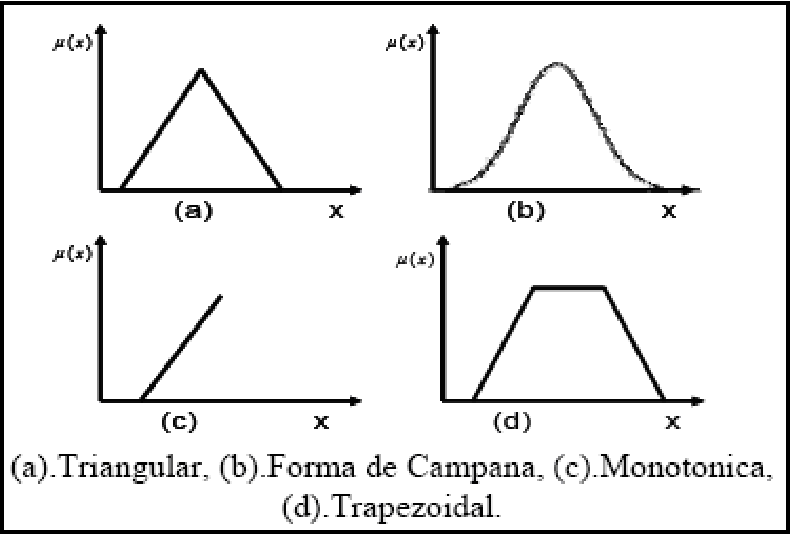
\includegraphics[width=0.5\linewidth]{\funcionM}
        \caption{Funciones de membresia mas comunes.}
        \label{fig:funcionM}
    \end{figure}

    \subsection{Fuzzificación}
    El control difuso siempre involucra este proceso de Fuzzificación, esta operación se realiza en todo instante de tiempo, es la puerta de entrada al sistema de inferencia difusa. Es un procedimiento matemático en el que se convierte un elemento del universo de discurso(variable medida del proceso) en un valor en cada función de membresía a las cuales pertenece.

    \begin{figure}[H]
        \centering
        \includegraphics[width=0.8\linewidth]{\fuzzy}
        \caption{Fuzzificación de una variable.}
        \label{fig:fuzzyV}
    \end{figure}

    Para comprender mejor veamos la figura~\ref{fig:fuzzyV} que arroja los siguientes datos:

    \begin{align}
        \mu_{\text{BAJOS}}(55) &= 0.25 \\
        \mu_{\text{REGULAR}}(55) &= 0.75 \\
        \mu_{\text{ALTOS}}(55) &= 0.00
    \end{align}

    El valor de velocidad igual a 55 pertenece a dos conjuntos con distintos grados en cada uno.
    A partir de ahora y durante el resto de las operaciones en el interior del corazón fuzzy estos datos (0.25, 0.75 y 0.00, son valores de las funciones de membresía) representarán a las variables censados del proceso. A tales datos les llamaremos $\mu$ en sentido genérico para diferenciarlos de otras funciones de membresía $\mu_A(x) = \mu$.


    \subsection{Mamdani.}
    Las reglas difusas de Mamdani son esenciales en sistemas de lógica difusa y controladores borrosos, modelando decisiones en entornos con imprecisión. Siguiendo la estructura "si-entonces", expresan condiciones y acciones en términos lingüísticos como "bajo" o "alto". Cada variable lingüística tiene funciones de membresía asociadas. Operaciones borrosas como "y" y "o" combinan condiciones en reglas ponderadas por su activación, definiendo el conocimiento del sistema. La inferencia difusa calcula la salida ponderadamente, y la defusificación convierte la salida difusa en un valor concreto para acciones. Estas reglas son versátiles, aplicándose en control difuso y toma de decisiones en contextos desafiantes para la precisión convencional.

    \subsection{defusificación.}
    La defusificación es la etapa crucial en un sistema de lógica difusa donde la salida difusa, expresada en conjuntos difusos, se convierte en un valor concreto para la toma de decisiones. Después de la inferencia difusa, que produce conjuntos difusos de salida, la defusificación busca resumir esta información en un valor numérico. Métodos comunes incluyen el uso del centro de gravedad, que encuentra el punto central ponderando los valores de salida por sus grados de membresía, y el método del valor máximo, que selecciona el valor máximo del conjunto difuso de salida como el resultado. La elección del método depende del contexto de la aplicación y los requisitos de precisión, siendo la defusificación esencial para traducir la información difusa en acciones o valores concretos en aplicaciones prácticas.

    
    \section{Metodología.}
    Para el desarrollo del sistema se utilizó Matlab con el paquete “MATLAB Support Package for Arduino Hardware”  para poder hacer uso de la placa arduino uno como interfaz de adquisición de datos de los sensores además de poder mandar los valores de las salidas a los actuadores, también se hace uso “Fuzzy logic toolbox”, con el cual se hizo la creación de la lógica difusa, a través de la interfaz gráfica que brinda ella paqueteria se pudo desarrollar el siguiente código~\ref{lst:fis}.
    %\clearpage
    \lstinputlisting[caption={Ejemplo de código MATLAB.}, label=lst:fis, title={ código 1 : Archivo del sistema de control difuso Mamdani}]{\codeB}

    Podemos observar en la figura~\ref{fig:completo} el modelo completo utilizado en el diseño.

    \begin{figure}[H]
        \centering
        \includegraphics[width=0.8\linewidth]{\sCompleto}
        \caption{Sistema difuso completo}
        \label{fig:completo}
    \end{figure}

    Se tiene como entrada los valores proporcionados por una resistencia variable LDR, así como un termistor, los cuales son encargado de sensar las condición relevante para el sistema y en función de los parámetros, que dependiendo del valor de entrada adecuado que se encontró se presentan los valores de entrada, donde como se aprecia en la figura~\ref{fig:nter} las escalas son distintas esto varía en función de los datos adquiridos durante las pruebas del sistema y determinación de que estos son los valores donde a nosotros nos convenía la activación o determinación de las variables lingüísticas de este sistema, ya que como se dijo de manera recurrente el sistema, gracias a esta interfaz gráfica se puede modificar de una maner a simple al variar estos valores y tener su propio conjunto de reglas difusas para adecuarse al ambiente o necesidades para cumplir con sus objetivo a través de este sistema.

    \begin{figure}[H]
        \centering
        \begin{subfigure}{0.8\linewidth}
            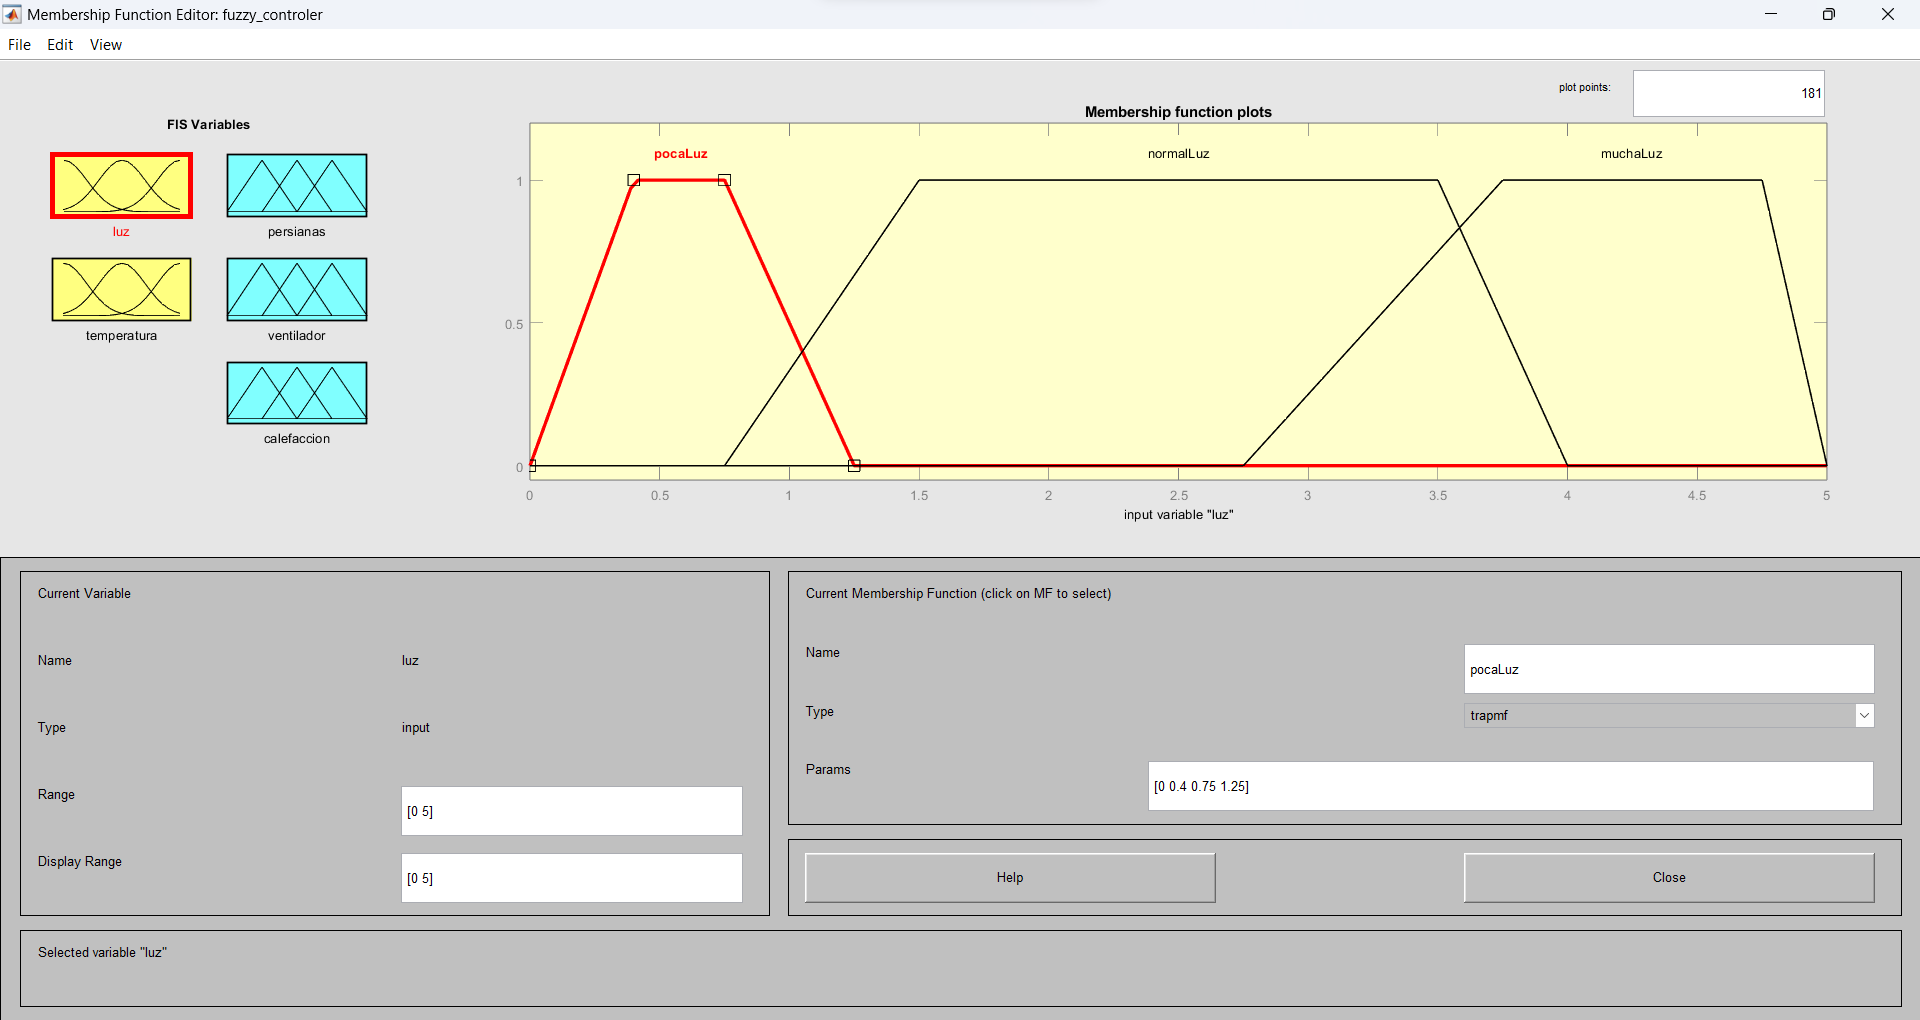
\includegraphics[width=\linewidth]{\luz}
            \caption{Conjunto difuso luz}
            \label{sub:luz}
        \end{subfigure}
        \begin{subfigure}{0.8\linewidth}
            \includegraphics[width=\linewidth]{\temperatura}
            \caption{Conjunto difuso temperatura}
            \label{sub:temp}
        \end{subfigure}
        \caption{Entradas}
        \label{fig:nter}
    \end{figure}

    Las salidas del sistema se puede considerara cualquier actuador, para simplificación de este sistema se colocaron leds en las pruebas y la intensificación de este es donde se determinó cual es el valor adecuado de dichas salidas, la interacción con motores o demás actuadores se puede considera para un paso final donde se realice una etapa intermedia (si así lo requiere) para obtener un correcto funcionamiento de dicha salida, de igual manera en la figura~\ref{fig:out} se pueden apreciar los valores que se determinaron para el funcionamiento de este sistema.

    \begin{figure}[H]
        \centering

        \begin{subfigure}{0.8\linewidth}
            \includegraphics[width=\linewidth]{\persianas}
            \caption{Conjunto difuso de las persinas}
            \label{sub:per}
        \end{subfigure}

        \begin{subfigure}{0.8\linewidth}
            \includegraphics[width=\linewidth]{\ventilador}
            \caption{Conjunto difuso de el ventilador}
            \label{sub:vent}
        \end{subfigure}

        \begin{subfigure}{0.8\linewidth}
            \includegraphics[width=\linewidth]{\calefacion}
            \caption{Conjunto difuso la calefacción }
            \label{sub:cale}
        \end{subfigure}

        \caption{Salidas}
        \label{fig:out}
    \end{figure}

    Considero de particular interés el hecho de que se tiene por decir de alguna manera 2 tipos de códigos, el que determina todo lo explicado hasta ahora, es decir la fase del control difuso a tavares del procesamiento de todos los datos adquiridos directamente de los puertos de la conexiones de arduino, pero ademas tenemos el codigo~\ref{lst:matlab} que define las propias acciones de arduino, esto lo considero de esta manera ya que tenemos diferentes etapas, que denominaría yo para el uso simple, ya que en el análisis de resultados no hay mayor complejidad al observar el sistema, pero el trasfondo de este sistema es eso que considero interesante, ya que para el usos particular del microcontrolador no se requiere hacer un manejo de registros con un lenguaje de bajo de bajo nivel, si no que hay una abstracción y en pocas lineas de código se puede lograr esto, anteriormente, se trató de implementar un sistema con Python, el cual fue la causa de que me diera cuenta de esta parte, ya que como se dijo de alguna manera se pueden considerar etapas intermedias unidas a través de \emph{“algo”}, que en este caso es el propio Matlab, lo que simplifica aun  mas las cosas, pero puede dejar de lado todo lo que existe debajo para esta implementacion final.

    \lstinputlisting[caption={Ejemplo de código MATLAB.}, label=lst:matlab, title={ código 2: Script Matlab }]{\codeA}
    En última instancia se deja una explicación de los puntos claves de las pocas líneas de código implementadas para el funcionamiento y conjunción de la placa arduino.

    \begin{itemize}

        \item Inicialización de Arduino: Se inicia la conexión con Arduino mediante el uso de la función `arduino()` y se asigna a la variable `a`.
        \item Configuración de Sensores y Actuadores: Se especifican los pines utilizados para los sensores de luz y temperatura (`light\_sensor` y `temp\_sensor` respectivamente), así como los actuadores como persianas (`blinds`), un ventilador (`fan`), y un componente para controlar la temperatura (`temp`).
        \item Bucle Principal (While): Se establece un bucle infinito (`while 1`) para mantener la ejecución continua del sistema.
        \item Lectura de Sensores: Se utilizan las funciones `readVoltage` de Arduino para medir los voltajes provenientes de los sensores de luz y temperatura (`volt\_light` y `volt\_temp` respectivamente).
        \item Carga del Controlador Difuso (FIS): Se carga el controlador difuso desde un archivo FIS (Sistema de Inferencia Difusa) utilizando la función `readfis`.
        \item Evaluación del Controlador Difuso: Se utiliza la función `evalfis` para evaluar el controlador difuso con los valores de entrada proporcionados por los sensores (`volt\_light` y `volt\_temp`).
        \item Modificación de las salidas: Se utiliza la salida del controlador difuso (`x`) para controlar los actuadores. En este caso, se ajusta la posición de las persianas (`writePosition`), la velocidad del ventilador (`writePWMDutyCycle`), y la tensión de un componente para controlar la temperatura (`writePWMVoltage`).
        
    \end{itemize}

    Como resultado este código representa un sistema de control difuso en tiempo real que ajusta la posición de las persianas, la velocidad del ventilador y la temperatura según las condiciones de luz y temperatura detectadas por los sensores.
    

    \section{Análisis de resultados.}
	Una vez establecido el diseño, los conjuntos y las reglas para el controlador se realizan los cálculos necesarios para obtener los valores de pertenencia, con estos y usando las reglas del controlador podemos obtener los resultados de salida.

	\begin{figure}[!h]
		\centering
		\includegraphics[scale=0.5]{\imgA}
		\caption{Gráfico en el comportamiento del controlador difuso.}
	\end{figure}

	Por cada una de las reglas se van analizando las relaciones de pertenencia a las que corresponden sus respectivas entradas y estas se van uniendo en la gráfica final en la que se obtendrá la figura final y en ella se tomará su centroide el cual será la salida a sus correspondientes dispositivos.\newline \\
	Con ayuda de la gráfica se aprecia que las salidas del controlador se van adaptando cada vez que se hace un cambio de modo que se obtiene de forma automática un valor adecuado según cada situación.\newline \\
	En el siguiente gráfico se observa como el controlador va tomando los valores de entrada tras calcular los valores de pertenencia determina en que situación se encuentra el entorno de modo que puede aumentar la apertura de las persianas para captar más luz además de determinar que la temperatura es adecuada por lo que buscará mantenerla en el mismo valor.

	\begin{figure}[!h]
		\centering
		\includegraphics[scale=0.5]{\imgB}
		\caption{Resultados al tomar entradas de poca luz y a baja temperatura.}
	\end{figure}
    
    En última instancia se hizo la implementación física del sistema que se muestra en la figura~\ref{fig:fisico} con un LDR un termistor, un servomotor y un motor dc de 5v, todos conectados a la placa y se verificó el correcto funcionamiento con esta implementación, los cuales dieron una respuesta satisfactoria a todas las proposiciones del sistema, lo cual no permitió interactuar con el entorno, el ensamble no es el mejor de manera estética, pero solo se deseaba probar el funcionamiento de lo propuesto durante todo este proyecto, a fin de cuentas debido a su flexibilidades puede ser implementado sobre diferentes situaciones que se pueden adaptar y con actuadores diversos haciendo las modificaciones para el acoplamiento satisfactorio.

	\begin{figure}[!h]
		\centering
		\includegraphics[width=\textwidth,height=10cm, keepaspectratio]{\implementacion}
		\caption{Sistema fisico implementado}
        \label{fig:fisico}
	\end{figure}

    \section{Conclusión}
    La flexibilidad inherente a la lógica difusa se ha demostrado en la capacidad del sistema para adaptarse a una variedad de situaciones y preferencias del usuario, sin la delimitación de un modelo matemático o un sistema bien definido, lo cual nos da  la posibilidad de ajustar fácilmente los conjuntos difusos así como las reglas que permite una personalización efectiva del sistema para diferentes escenarios adaptándose a las necesidades específicas de un entorno, también se puede destacar que a través de la validación en conjunto con la prueba del sistema en tiempo real han confirmado su capacidad para tomar decisiones de manera autónoma, respondiendo de manera coherente a las condiciones cambiantes del entorno en función de las reglas difusas que se generaron, se puede destacar la inteligibilidades que nos brinda las variables lingüísticas, comentar que siendo honestos se tienen palabras abstraídas siempre en todo contexto y que solo se requiere entender el funcionamiento o hacer la homologación se su funcionamiento a algo similar que entendamos mejor, para permitirnos realizar una fácil implementación de todo lo propuesto en este trabajo; lo anterior se puede notar en los conceptos como la fuzzificacion o la defusificación, que en conjunto han sido cruciales para convertir las salidas difusas en acciones tangibles y comprensibles, permitiendo una interacción efectiva con el entorno físico. Con lo cual en resumen, este proyecto ha demostrado que la lógica difusa Mamdani es una herramienta poderosa para el control adaptativo en entornos variables, a la vez que nos permitió ahondar más del tema para comprender la capacidad de modelar la imprecisión inherente en las condiciones ambientales, conjuntando con la flexibilidad para ajustarse a diversas situaciones que respaldan la utilidad de la lógica difusa en aplicaciones prácticas de control. Este enfoque contribuye significativamente a la creciente demanda de sistemas inteligentes y adaptables en diversos contextos, desde entornos domésticos hasta aplicaciones industriales.
\end{document}
